\chapter{Results}
\label{chap:results}

\lettrine[lines=4, findent=3pt, nindent=0pt]{I}{n} this chapter results and performance will be discussed. Starting with some metrics about the trained \gls{ml} model, with a particular focus on grouped and ungrouped features, it will then be presented the behavior of the implemented \gls{ids} on real life attacks, taking into consideration what was pointed out in section \ref{subsec:delimitation} about the delimitation of the project. Anyway, the theoretical results achieved remain valid and for this reason form the focus of the chapter.

\section{ML Model Evaluation}
\label{sec:ml-model-evaluation}

The classifier of choice, as discussed in \ref{subsec:classification}, was \textit{Random Forest}. It is particularly interesting to observe the results of the training with ungrouped labels versus the one with grouped labels: the differences in terms of precision and F1 score are remarkable.

% \begin{figure}[h!]
%    \centering
%    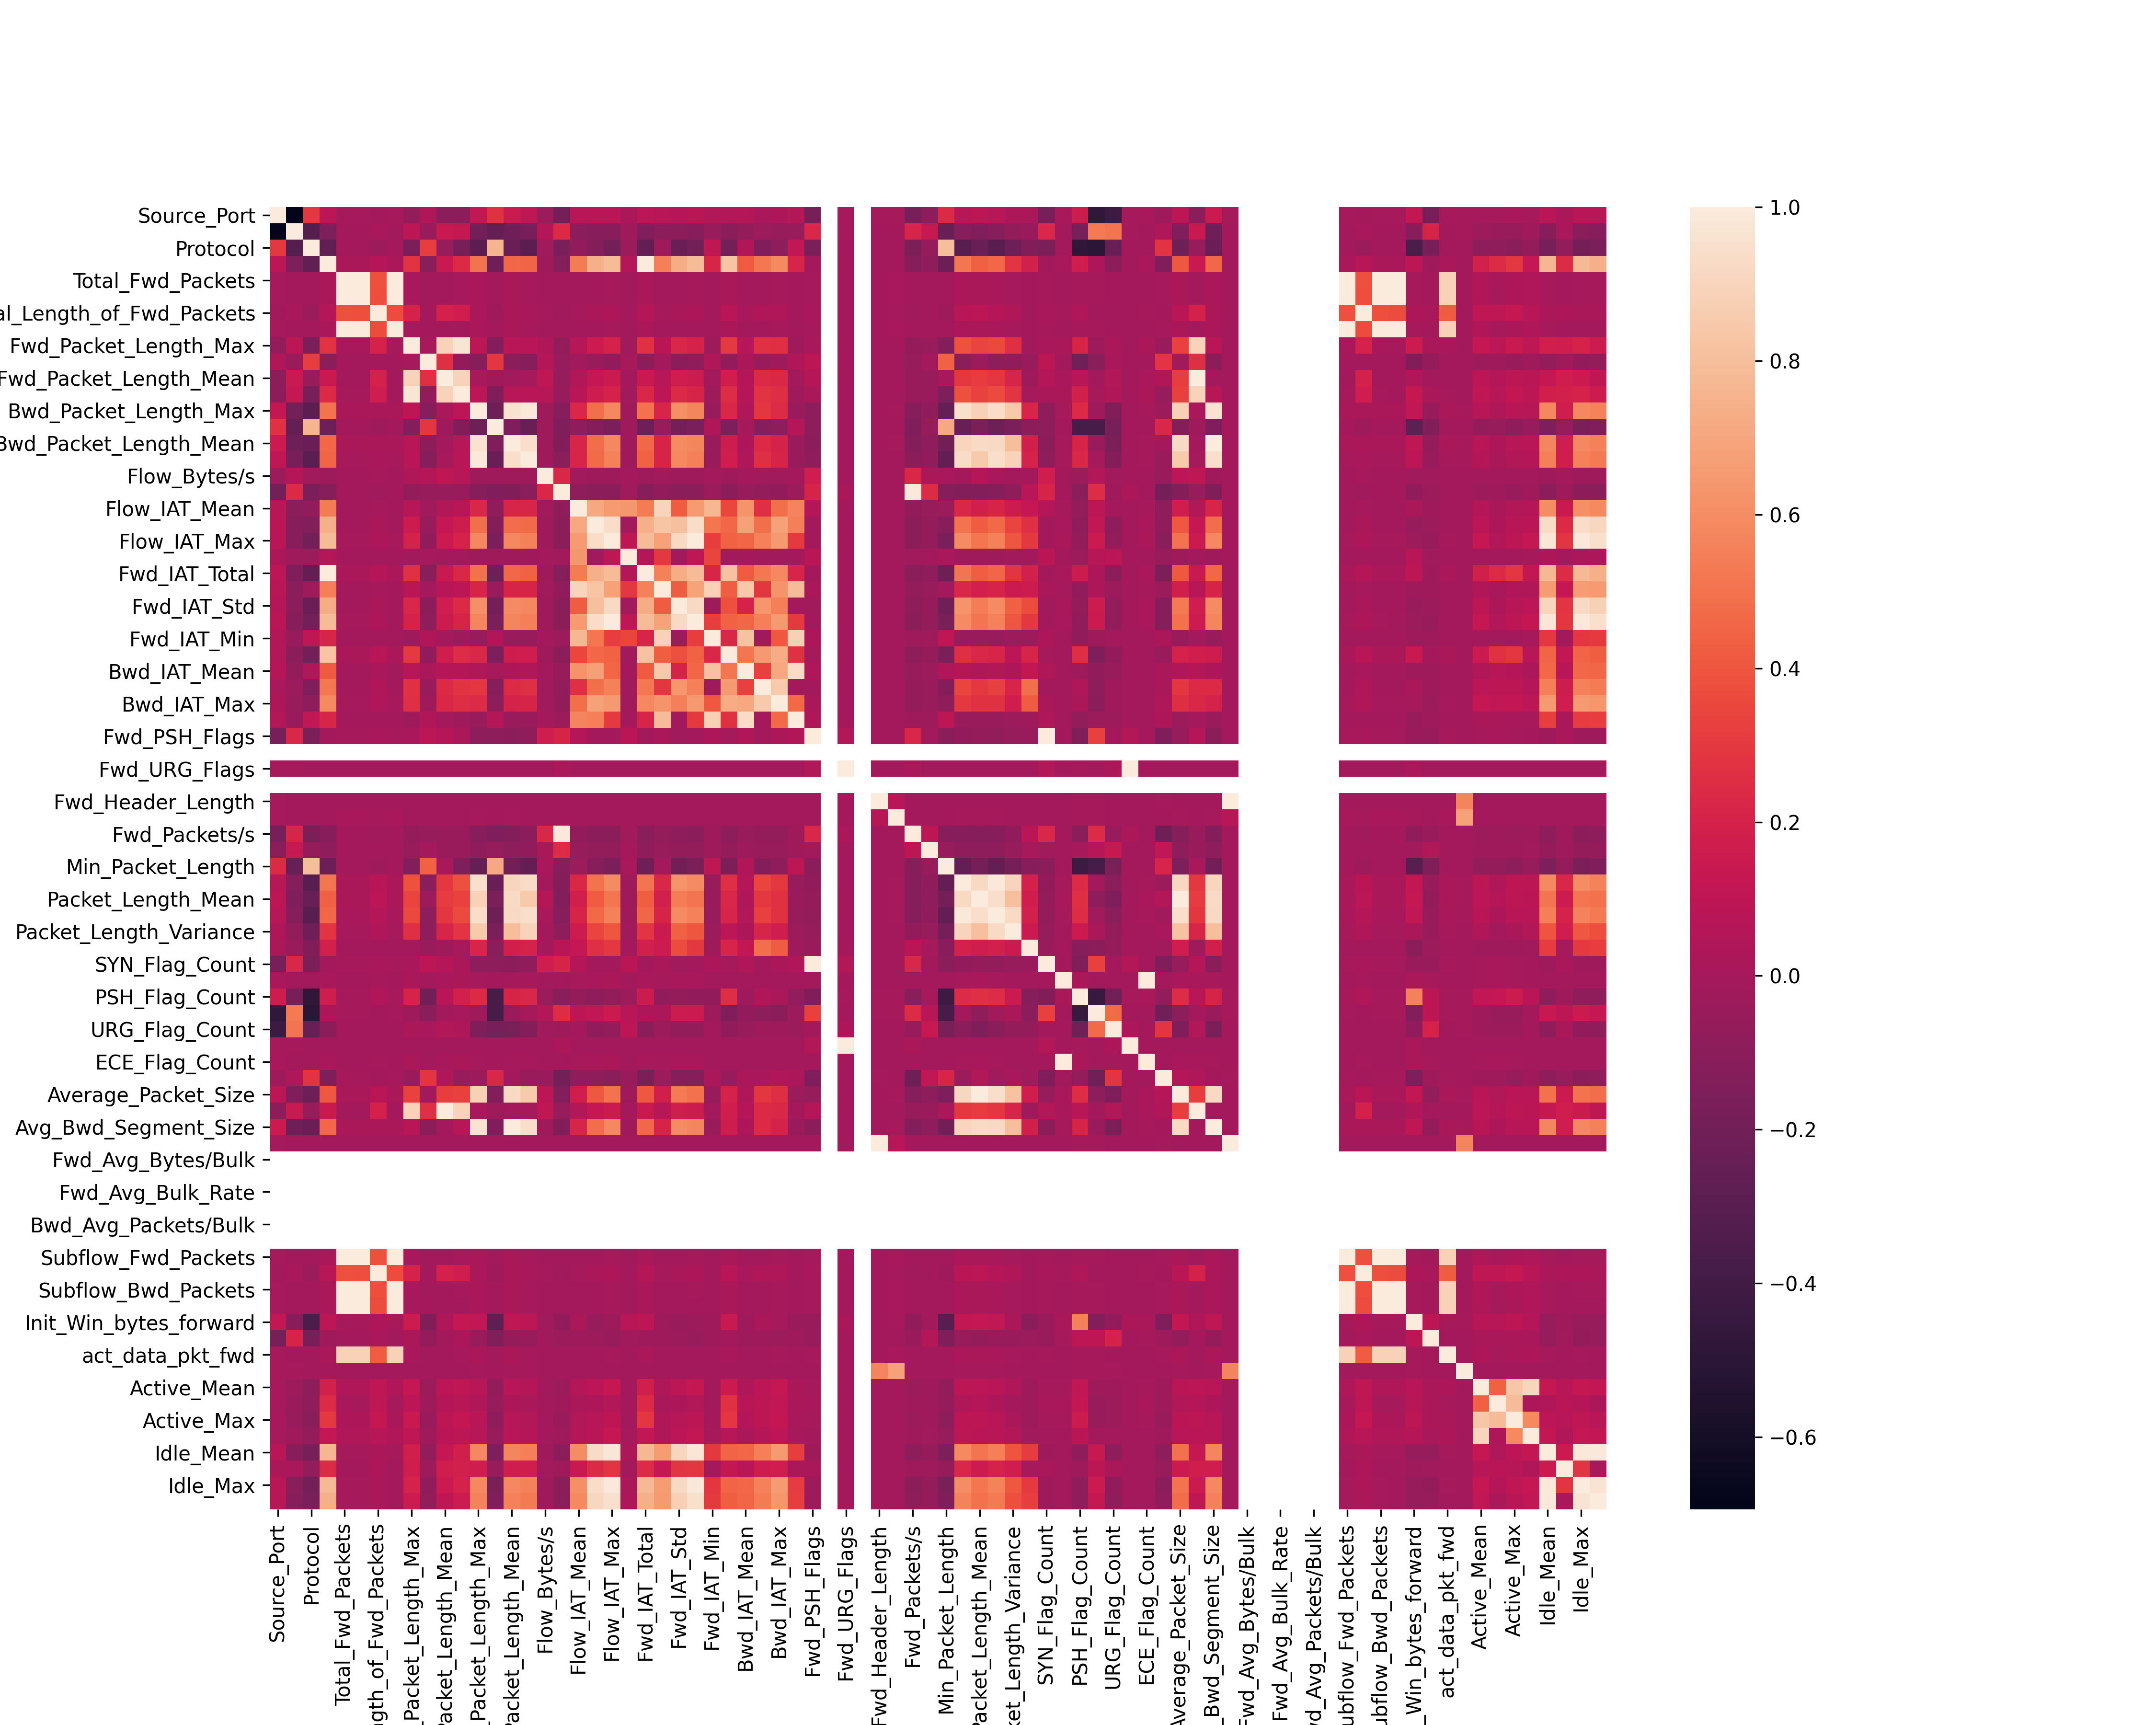
\includegraphics[scale=0.5]{assets/figures/chapter3/heatmap-all.png}
%    \caption{CICIDS2017 Feature Correlation Matrix (heatmap)}
%    \label{fig:feature-heatmap}
% \end{figure}

\subsection{Ungrouped Labels Model}
\label{subsec:ungrouped-training}

Considering the model trained with all the labels available in the dataset, performance is expected to be lower that the one trained on grouped features. Three metrics will be considered for the comparison of the features (\textit{precision}, \textit{recall} and \textit{F1 score}).
\par Table \ref{tab:ungrouped-metrics} shows the metrics achieved by the model, regarding each feature. The average \textit{precision} is $90.9253\%$, the average \textit{recall} is $88.1413\%$ and the average \textit{F1 Score} is $89.2012\%$, with an overall \textit{accuracy} of $99.8636\%$. The training time was $802.53$ seconds, using the hardware listed in \ref{sec:model-training} and training the model on a Jupyter Notebook using Python \texttt{3.9.4} (64-bit).

\begin{table}[h!]
   \centering
   \begin{tabular}{l|llll}
       \toprule 
       Traffic Label & Precision (\%) & Recall (\%) & F1 Score (\%) \\
       \midrule
       \rowcolor{black!10} \texttt{Benign} & 99.9480 & 99.9219 & 99.9349 \\
       \texttt{Bot} & 84.1463 & 52.9412 & 64.9922 \\
       \rowcolor{black!10} \texttt{Brute Force} & 72.3602 & 77.4086 & 74.7994 \\
       \texttt{DDoS} & 100.0000 & 99.9570 & 99.9785 \\
       \rowcolor{black!10} \texttt{DoS GoldenEye} & 99.9023 & 99.4169 & 99.6590 \\
       \texttt{DoS SlowHTTPTest} & 99.0036 & 99.3636 & 99.1833 \\
       \rowcolor{black!10} \texttt{DoS Hulk} & 99.6793 & 99.9565 & 99.8177 \\
       \texttt{DoS Slowloris} & 99.8261 & 99.0509 & 99.4370 \\
       \rowcolor{black!10} \texttt{FTP-Patator} & 100.0000 & 99.8740 & 99.9369 \\
       \texttt{Port Scan} & 99.4457 & 99.9748 & 99.7095 \\
       \rowcolor{black!10} \texttt{SSH-Patator} & 100.0000 & 99.8305 & 99.9152 \\
       \texttt{XSS} & 36.7925 & 30.0000 & 33.0508 \\
       \bottomrule
   \end{tabular}
   \caption{\textit{Random Forest} trained model metrics on CICIDS2017 (ungrouped) features}
   \label{tab:ungrouped-metrics}
\end{table}

Although the shown results are not bad, they are certainly lowered by the \texttt{Bot}, \texttt{Brute Force} and \texttt{XSS} attacks classification, and this comes also clear form the \textit{confusion matrix} displayed in figure \ref{fig:ungrouped-confusion-matrix}: some of the \texttt{Bot} attacks are classified as \texttt{Benign}, some of the \texttt{Brute Force} ones are classified as \texttt{XSS} and vice versa; the problem is the proportion in which the classification goes wrong (\textit{e.g.: DoS Hulk has been classified 46005 times correctly and 137 times as benign traffic, while XSS has been classified 39 times correctly and 66 times as a brute force attack}). A possible explanation regarding the poor classification performance on these attacks can be maybe that features that correctly identify said attacks are not in the \textit{transport layer}, but in the \textit{application} one, such as particular characters used, or cookie payload, for example.

\begin{figure}[h!]
   \centering
   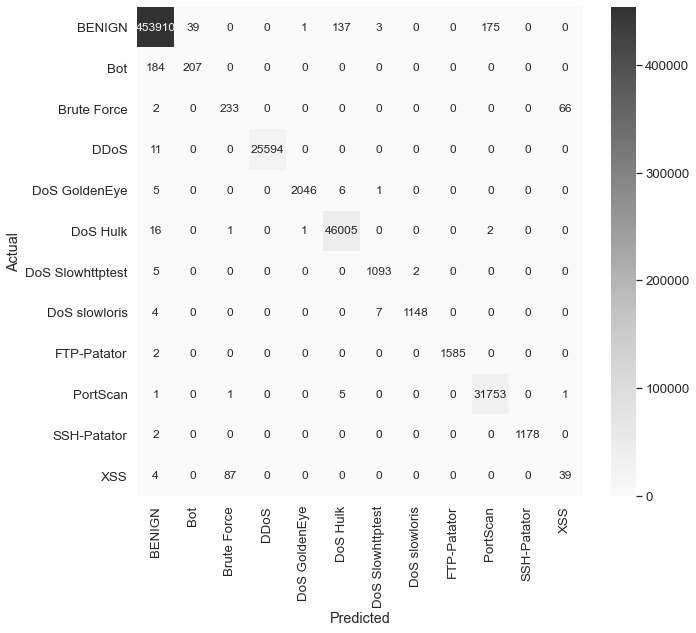
\includegraphics[scale=0.62]{assets/figures/chapter3/ungrouped_confusion_matrix.png}
   \caption{Confusion Matrix of the \textit{Random Forest} model trained using CICIDS2017 dataset (ungrouped) features}
   \label{fig:ungrouped-confusion-matrix}
\end{figure}

\subsection{Grouped Labels Model}
\label{subsec:grouped-training}

Due to the variability of network attacks, always changing and updating, it is more important to identify the category of said malicious traffic, rather than the specific tool used to generate it. For this reason the features concerning specific attacks were grouped: this helps with generalization and reliability of the trained model, since the classification takes place observing different attacks, all with the same purpose (\textit{e.g. Information Gathering, Stress Testing, etc.}).
\par Contrary to the considerations made in section \ref{subsec:ungrouped-training} for the ungrouped training, the expectations for the model trained with the grouped labels are higher. For obvious reasons the metrics used are the same used in the previous section (\textit{precision}, \textit{recall} and \textit{F1 Score}); the model is presumed to perform significantly better then the first one.
\par As highlighted in section \ref{subsec:pre-processing}, the 12 traffic types can be grouped into 7 bigger categories, leading to less labels to predict and, hopefully, less classification errors. Table \ref{tab:grouped-metrics} displays the metrics for each of said categories. The average \textit{precision} is $97.9827\%$, the average \textit{recall} is $95.9278\%$ and the average \textit{F1 Score} is $96.8638\%$, with an overall \textit{accuracy} of $99.9089\%$. The training time, using the same hardware and software as before, was completed in $760.18$ seconds.
\par From the data collected, the model has performed as expected: all three metrics increased significantly while the training time has decreased, resulting in a better performing model.

\begin{table}[h!]
   \centering
   \begin{tabular}{l|llll}
       \toprule 
       Traffic Label & Precision (\%) & Recall (\%) & F1 Score (\%) \\
       \midrule
       \rowcolor{black!10} \texttt{Benign} & 99.9681 & 99.9208 & 99.9444 \\
       \texttt{Botnet} & 87.4618 & 73.1458 & 79.6657 \\
       \rowcolor{black!10} \texttt{Brute Force} & 100.0000 & 99.9277 & 99.9638 \\
       \texttt{DDoS} & 100.0000 & 99.9727 & 99.9863 \\
       \rowcolor{black!10} \texttt{DoS} & 99.7047 & 99.9404 & 99.8224 \\
       \texttt{Probe} & 99.4456 & 99.9717 & 99.7080 \\
       \rowcolor{black!10} \texttt{Web Attack} & 99.2991 & 98.6079 & 98.9523 \\
       \bottomrule
   \end{tabular}
   \caption{\textit{Random Forest} trained model metrics on CICIDS2017 (grouped) features}
   \label{tab:grouped-metrics}
\end{table}

Comparing the \textit{confusion matrix} shown in figure \ref{fig:grouped-confusion-matrix} to the previous one, it is clear that some problems regarding the \texttt{Botnet} label remain, in fact it is the only one performing poorly also in this scenario. As discussed above, one way to fix this is by changing methodology, observing the network traffic at \textit{application level}, modifying the considered features, since from \textit{transport level} botnet's traffic can blend with the normal traffic, resulting in being classified as \texttt{Benign}.

\begin{figure}[h!]
   \centering
   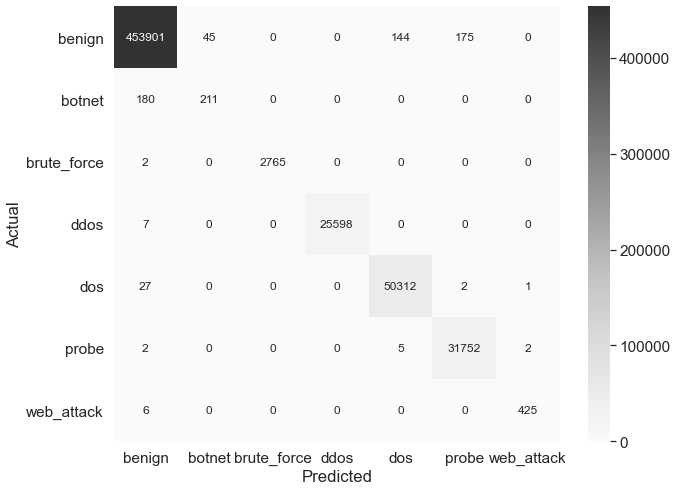
\includegraphics[scale=0.52]{assets/figures/chapter3/grouped_confusion_matrix.png}
   \caption{Confusion Matrix of the \textit{Random Forest} model trained using CICIDS2017 dataset (grouped) features}
   \label{fig:grouped-confusion-matrix}
\end{figure}

To summarize the advantages of using grouped labels, table \ref{tab:grouped-vs-ungrouped} shows the increase of all the metrics concerning the reliability of the model and, at the same time, the decrease of the training time.

\begin{table}[h!]
   \centering
   \begin{tabular}{l|lllll}
       \toprule 
       Type & Precision (\%) & Recall (\%) & Accuracy (\%) & F1 Score (\%) & Training Time (s) \\
       \midrule
       \rowcolor{black!10} All Labels & 90.9253 & 88.1413 & 99.8636 & 89.2012 & 802.5287 \\
       Grouped Labels & 97.9828 & 95.9278 & 99.9089 & 96.8638 & 760.1764 \\
       \midrule
       $\Delta$ & \faArrowAltCircleUp[regular] 7.0575 & \faArrowAltCircleUp[regular] 7.7865 & \faArrowAltCircleUp[regular] 0.0453 & \faArrowAltCircleUp[regular] 7.6626 & \faArrowAltCircleDown[regular] 42.3523 \\
       \bottomrule
   \end{tabular}
   \caption{Difference between trained models}
   \label{tab:grouped-vs-ungrouped}
\end{table}

\section{Attack Detection and Classification}
\label{sec:attack-detection}

The implemented \gls{ids} has been tested to check its behavior with real life attacks using both \textit{synchronous} and \textit{asynchronous} modes: in other words acquiring traffic from the L3 switch, or using \gls{pcap} files acquired separately (generated or downloaded from the internet).
\par The \textit{Random Forest} classifier was able to identify the attacks on which has been trained on: \texttt{Botnet}, \texttt{Brute Force}, \texttt{DDoS}, \texttt{DoS}, \texttt{Probe} and \texttt{Web Attacks}. As mentioned above, the attacks were either generated by the tools discussed in \ref{subsec:pentesting-tools} or pre-packaged in a \gls{pcap} file downloaded form the internet (usually datasets). Table \ref{tab:attack-predictions} summarizes well the attacks performed and the associated prediction.

\begin{table}[h!]
   \centering
   \begin{tabular}{l|lll}
       \toprule 
       Tool Used & Generated Attack & Prediction & \\
       \midrule
       \rowcolor{black!10} Patator & SSH Brute Force & \texttt{Brute Force} & \faCheck \\
       Patator & FTP Brute Force & \texttt{Brute Force} & \faCheck \\
       \rowcolor{black!10} SlowHTTPTest & Stress Test & \texttt{DoS} & \faCheck \\
       SlowLoris & Stress Test & \texttt{DoS} & \faCheck \\
       \rowcolor{black!10} NMap & Information Gathering & \texttt{Probe} & \faCheck \\
       ISCX-Bot-2014 Dataset & Botnet & \texttt{Botnet} & \faCheck \\
       \bottomrule
   \end{tabular}
   \caption{Generated attacks and associated prediction}
   \label{tab:attack-predictions}
\end{table}
\textit{ISCX-Bot-2014} is a dataset used to check, as the name suggests, if the \gls{ids} was able to detect botnets. It was provided by the \textit{Canadian Institute for Cybersecurity} \cite{Beigi2014}, just like the dataset used for the training.
\par No further analysis were conducted, since the only purpose of this test was to check the functionality of the \gls{poc}, not to recalculate the metrics discussed in section \ref{subsec:grouped-training}.